\documentclass[10pt,a4paper]{article}
\usepackage[latin1]{inputenc}
\usepackage{amsmath}
\usepackage{amsfonts}
\usepackage{amssymb}
\usepackage{graphicx}
\usepackage{float}
\author{Michele De Vita}
\begin{document}
	\begin{enumerate}
		\item If \textit{age} increase from 25 to 26 when all other variables are the same we have an increase of \textit{ahe} of 0.31. The same for 33 to 34.
		\item  If \textit{age} increase from 25 to 26 when all other variables are the same we have an increase of \textit{ahe} of $ 2\% $. The same for 33 to 34.
		\item In this case has no sense explain the \textit{age} increase from 25 to 26 because we used a log-log scale that explain the increase by $ 1\% $ of age and not by $ 1 $ unit. If we want to interpreter the coefficient before $ age $ we can say that if age increase by $ 1\% $,  $ ahe $  increase by $ 0.006369 $
		\item Since when $ age  $ increase by one the variable $ age^2 $ also increase we cannot interpreter the coefficient before $ age $
		\item Between the 3 and 2 we prefer the 2 because the explain the increase of $ age $ by 1 $ unit $ instead of $ 1\% $ 
		\item We prefer the 2 because the 4 with $ age^2 $ doesn't explain anything more than 2
		\item We prefer the 3 for the same reason of the point 5 of this exercise
		\item 
		\begin{figure}[H]
			\centering
			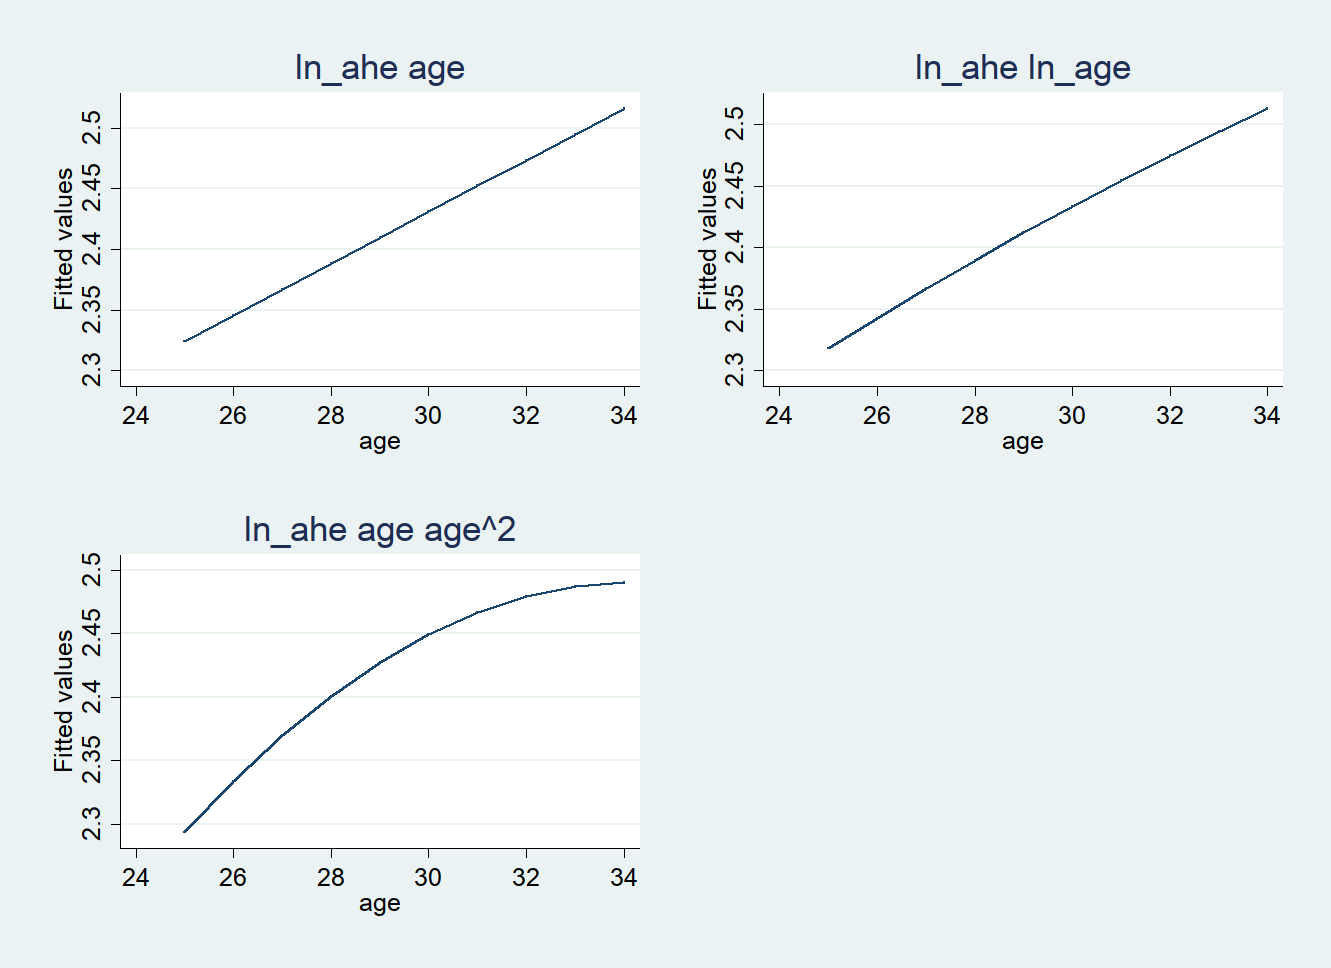
\includegraphics[width=0.7\linewidth]{plot_3_regressions}

		\end{figure}
		
	\end{enumerate}
\end{document}